\documentclass[main]{subfiles}


\begin{document}
\newpage
\section{Neuromorphic Systems 1}

\subsection{History and motivation}

\subsubsection{History}
Neuromorphic Engineering (NE) Neuromorphic engineering is a relatively young field that attempts to build physical realizations of biologically realistic models of neural systems using electronic circuits implemented in very large scale integration technology. The concept was coined by Carver Mead in the late 1980s. Carver Mead together with John Hopfield and Richard Feynmann started the Physics of Computation course at Caltech, which later transformed to the fully-flagged Phd/MSc program called "Computation and Neural Systems". Notable alumni are INI professors like Tobi Delbruck, Shi-Chi Liu and Giacomo Indiveri. Carver Mead also coined Moore's Law:  the number of transistors in a dense integrated circuit doubles about every two years.

\subsubsection{Physical comparisons: channel vs. transistor}

NE is possible because the physics of voltage activated membrane channels and transistors are closely related. When MOSFETs are operated in the weak-inversion regime (sub-threshold), the main mechanism of carrier transport is that of diffusion, as it is for ions flowing through proteic channels across neuron membranes:

\begin{itemize}
    \item $K^+$ conductance of cell membrane increases exponentially with the membrane voltage, until it approaches saturation at the maximal opening of the channel.
    \item Drain-to-Source Current ($I_{DS}$) flowing through a MOS transistors increases exponentially with the Gate-to-Source Voltage ($V_{GS}$) below a specific "threshold" voltage and quadratically above this value.
\end{itemize}{}

%
\begin{figure}[h]
    \centering
    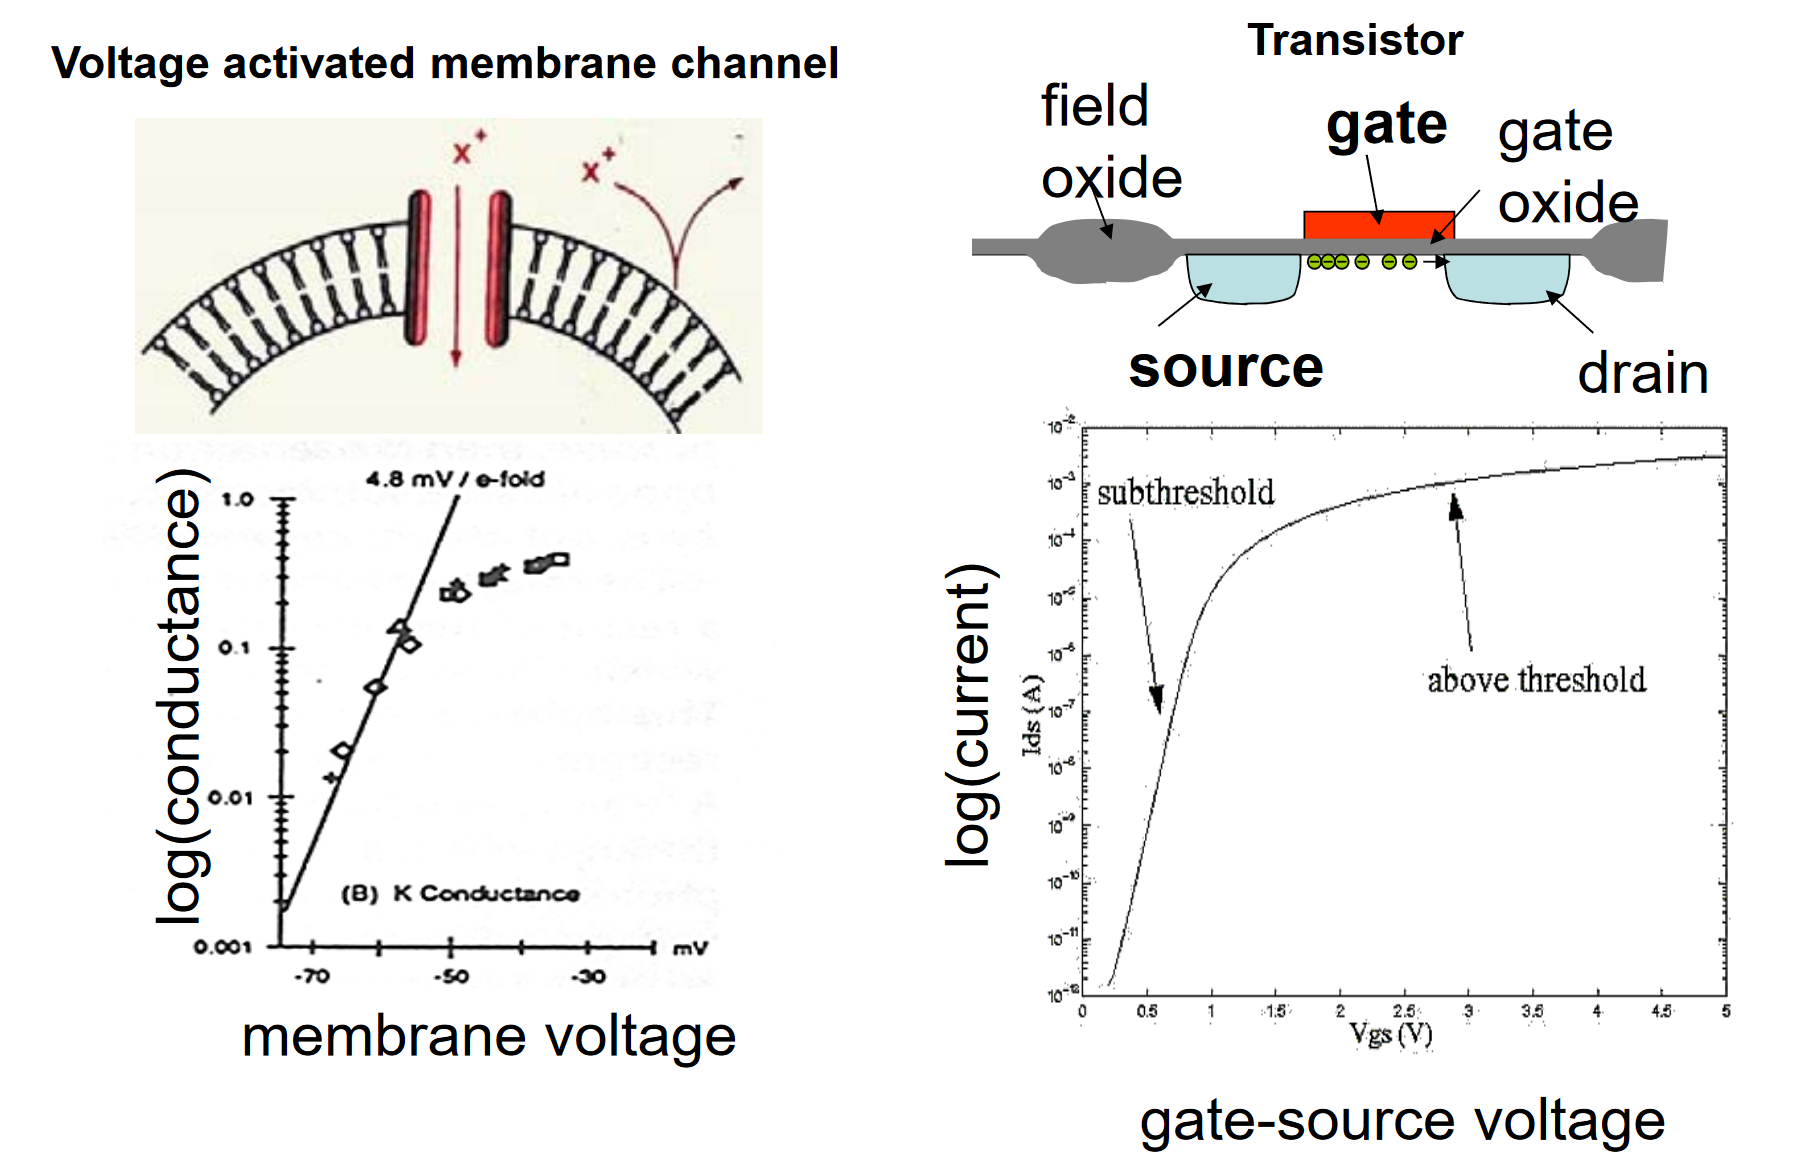
\includegraphics[width=0.8\linewidth]{11_NeuromorphicSystems1/figures/mem_vs_transist.PNG}
    \caption{Comparing a voltage activated membrane channel to the MOS transistor.}
    \label{fig:MEMvsTRANS}
\end{figure}
%

\subsubsection{Physical comparisons: brain vs. computer}
Even though conventional computation powered by silicon has seen immense gains in the past decades, as predicted by Moore's law, natural computation is still at least a million times more power efficient.

Some notable differences between brain-natural and artificial computation are presented below:

\begin{table}[h]
\begin{tabular}{|c|c|}
\hline
\textbf{Artificial Computation}         & \textbf{Brain}                                \\ \hline
Fast clocked system (GHz)               & Self-timed, data-driven (0.1 Hz to tens kHz)  \\ \hline
Bit-perfect deterministic logical state & Synapses are stochastic                       \\ \hline
Memory distant to computation           & Memory local to computation                   \\ \hline
High-bit resolution                     & Low-bit resolution with neurons as quantizers \\ \hline
\end{tabular}
\end{table}

\subsubsection{Physical comparisons: cell vs. ALU}
When looking at individual neuronal cells structurally we can define a set of computational steps executed by each main components:

\begin{itemize}
    \item \textbf{Channels} execute a form of multiplication as observed in Figure \ref{fig:MEMvsTRANS}.
    \item \textbf{Synapses} host populations of channels which open at the arrival of a PSP. The effect of each channel in the population is summed up, making the synapse behave like a Multiply-Accumulate unit.
    \item \textbf{Cell membrane} hosts complementary channels which can both increase the membrane voltage or decrease it.
    \item \textbf{Dendrites} connect to pre-synaptic neurons through both excitatory and inhibitory synapses, leading to analog additions and subtractions being executed at the level of single dendrites.
    \item \textbf{Dendritic trees} perform another level of analog computation, integrating the potentials arriving from each dendrite into the cell body.
    \item \textbf{Axons} transmit digital spike events (APs) to distant cells. 
\end{itemize}{}

\subsubsection{Neuromorphic VLSI circuits}

Detailed biophysical models of cortical circuits are derived from neuroscience experiments. Neural networks models are designed, with realistic spiking neurons and dynamic synapses, then mapped into analog circuits and integrated in large numbers on VLSI chips. [cite: computational intelligence book] 

One example of analog integrated circuit with the functional characteristics of real nerve cells can be seen in Figure \ref{fig:hh}. Because the physics underlying the conductivity of silicon devices and biological membranes is similar, the 'silicon neuron' is able to emulate efficiently the ion currents that cause nerve impulses and control the dynamics of their discharge. It operates in real-time and consumes little power, and many 'neurons' can be fabricated on a single silicon chip.  [cite: a silicon neuron] This neuron implements the Hodgkin-Huxley model which expresses the membrane conductance effects of $Na^+$ and $K^+$ ion currents and of the passive leak at rest and during an action potential. The variable conductance is implemented using the \textit{follower-integrator} circuit. The follower-integrator is composed of a transconductance amplifier configured in negative feedback mode with its output node connected to a capacitor. In weak-inversion the circuit behaves as a first-order low-pass filter with a tunable conductance. [cite neuromorphic silicon neurons].
%
\begin{figure}[h]
    \centering
    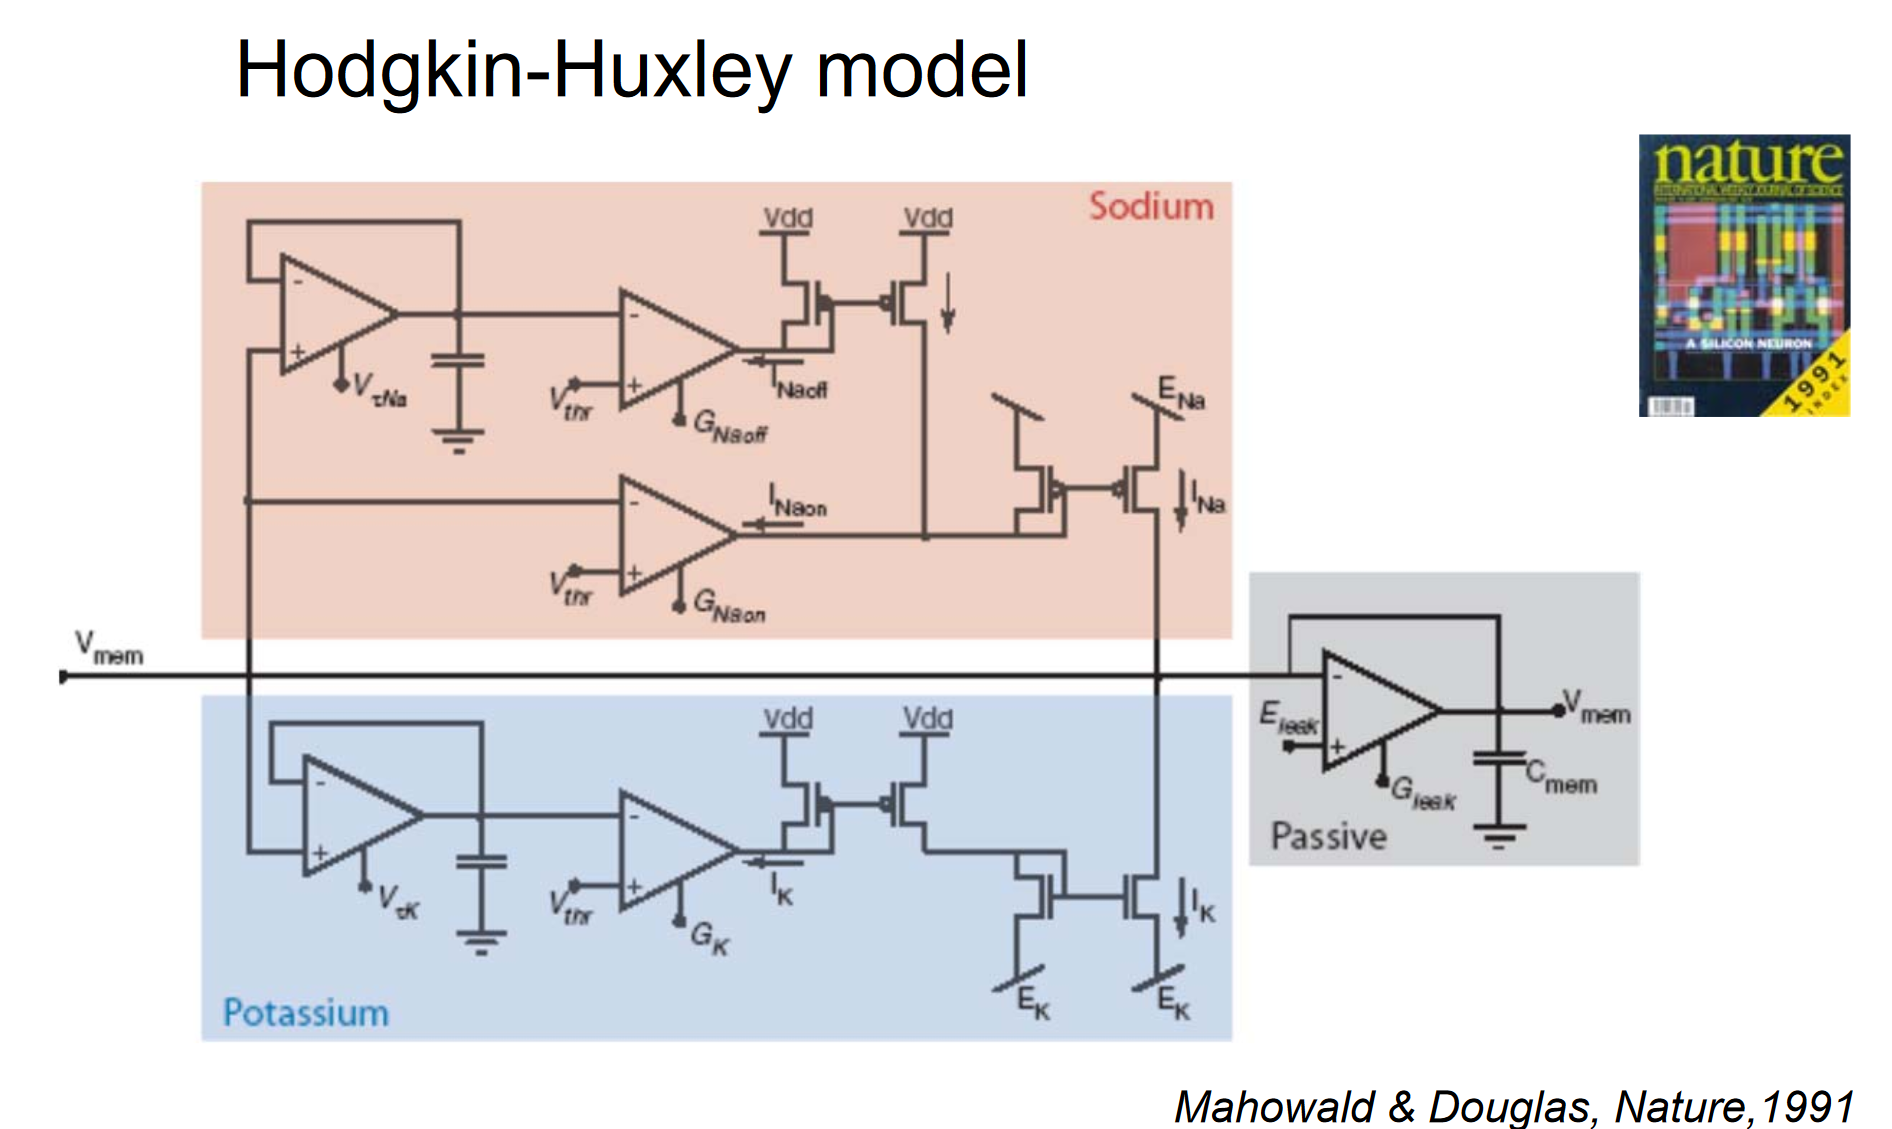
\includegraphics[width=0.8\linewidth]{11_NeuromorphicSystems1/figures/hh_model.png}
    \caption{A silicon neuron circuit.}
    \label{fig:hh}
\end{figure}
%

Processors harnessing both digital and analog techniques have been built in the past decade and they are presented in more detail in Lecture 12.

\subsection{Modelling vision and audition}
\subsubsection{Dynamic Vision Sensor: silicon retina}
The human retina contains around $10^8$ analog receptors, $10^6$ ganglion cells with spiking outputs and $10^9$ dynamic range modulating cells while consuming less than 3 mW of power. The retinal cone cells perform a special function of adjusting the operating point and the gain according to background illumination. This is driven by an active cell adaptation mechanism which is manifested as a shift in the light intensity-response curve, providing high sensitivity even in very low-light conditions. This property of the retina has inspired inventors in building state-of-the-art imaging sensors like the Dynamic Vision Sensor, whose main component, the Pixel, is depicted in Figure \ref{fig:dvs}.
%
\begin{figure}[h]
    \centering
    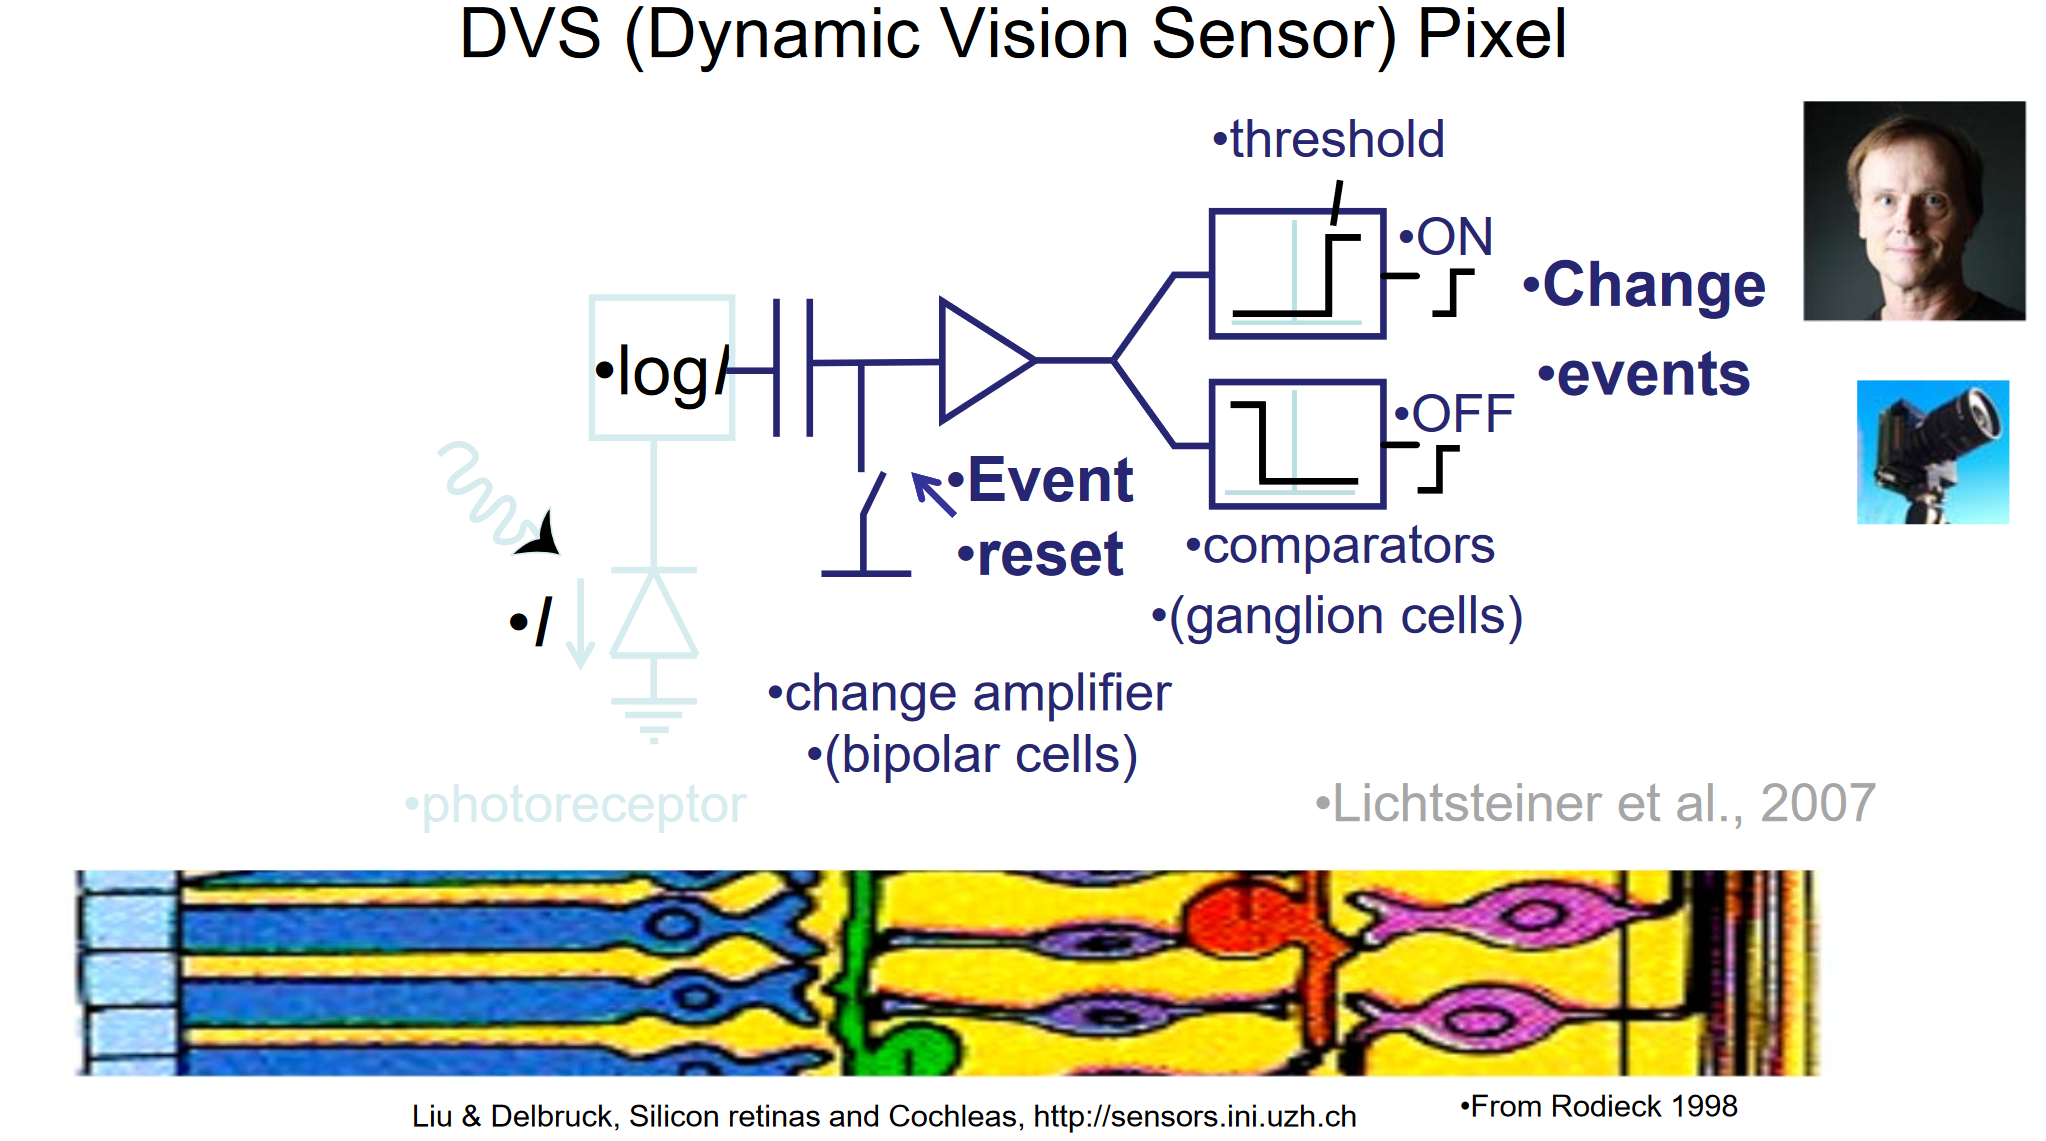
\includegraphics[width=0.8\linewidth]{11_NeuromorphicSystems1/figures/DVS.PNG}
    \caption{The Pixel.}
    \label{fig:dvs}
\end{figure}
%

The continuous-time front end photoreceptor (inspired from the adaptive photoreceptor) is the correspondent of the cone cell. The  photoreceptor  circuit  comprises  a  photodiode  whose photocurrent is sourced by a saturated NMOS transistor. This  well-known  transimpedance  configuration converts the photocurrent logarithmically into a voltage and also holds the photodiode clamped at a virtual ground. 

%[cite: http://siliconretina.ini.uzh.ch/wiki/lib/exe/fetch.php?media=lichtsteiner_dvs_jssc08.pdf]

The bipolar cell is built as a precision self-timed switched-capacitor differentiator. Local capacitor ratio matching gives the differencing circuit a precisely defined gain for changes in log intensity, thus reducing the effective imprecision of the comparators that detect positive and negative changes in log intensity. The DC mismatch is removed by balancing the output of the differencing circuit to a reset level after the generation of an event. 

The last stage is the comparison of the output of the inverting amplifier against global thresholds that are offset from the reset voltage to detect increasing and decreasing changes. If the input of a comparator overcomes its threshold, an ON or OFF event is generated. This part can be regarded as a ganglion cell and is build using cheap  two-transistor comparators.

Each pixel independently and in continuous time quantifies local relative intensity changes to generate spike events. These events appear at the output of the sensor as an asynchronous stream of digital pixel addresses. These address-events signify scene reflectance change and have sub-millisecond timing precision. This communication protocol is called Address-Event-Representation (AER). The output data rate depends on the dynamic content of the scene and is typically orders of magnitude lower than those of conventional frame-based imagers. 

The Dynamic and Active Pixel Vision Sensor (DAVIS) combines active pixel technology with the DVS temporal contrast pixel. The two streams of frames and events are output concurrently. That way, the DAVIS produces conventional frames, which are the basis of all existing machine vision, and the event stream that allows quick responses with sparse data and high dynamic range. [http://sensors.ini.uzh.ch/sensors-21.html]

Some demonstrative applications of the DVS/DAVIS are optical-flow, ultra-low power (2ms reaction at 4\% CPU usage) object tracking (RoboGoalie), autonomous driving and drone flight, high-speed robotics. 

An example algorithm used for object tracking with the DVS uses spatio-temporal coherence:
\begin{enumerate}
    \item For each event find nearest cluster
    \item If the event is withing the cluster, move the cluster, else send new cluster
    \item Periodically manage cluster lifetime
\end{enumerate}

\subsubsection{Dynamic Audio Sensor: silicon cochlea}

The Dynamic Audio Sensor is an asynchronous event-based silicon cochlea. The board takes stereo audio inputs and the custom chip asynchronously outputs a stream of address-events representing activity in different frequency ranges. As such it is a silicon model of the cochlea, the auditory inner ear. The system has also been called AER-EAR.

It uses cascaded second-order sections (SOS) to model the physical oscillation of the basilar membrane. These drive half-wave rectifier circuits, which model inner hair cells. These in turn drive multiple pulse frequency modulator circuits, which model ganglion cells with different spike thresholds. The resonance of individual sections can be adjusted with local digital-to-analog converters. 

This chip includes a variety of features including a matched binaural pair of cochleas, on-chip digitally controlled biases, on-chip microphone preamplifiers, and open-sourced host software APIs and algorithms. A bus-powered USB board enables easy interfacing to standard PCs for control and processing (Fig. 1), whilst a parallel AER port allows direct connection to other dedicated spiking neuromorphic hardware.

Each cochlea consists of a 64-stage cascaded filter bank stage. The cascaded architecture is preferred over a coupled bandpass architecture so we can achieve better matching and sharp high frequency roll-off. Each filter stage consists of a second-order-section (SOS) filter which is biased by a Complementary Lateral Bipolar Transistor (CLBT) ladder to improve matching [11]. A differential readout of each SOS output drives its own halfwave rectifier (HWR) circuit, and the HWR output drives 4 pulse-frequency modulators (PFMs). The PFM circuits implement an integrate-and-fire model with a threshold (VT). The four PFMs have individual global thresholds (VT1 to VT4), allowing volume encoding by selective activation of PFMs. Compared with regularly-sampled audio systems, the PFM outputs are transmitted asynchronously, reducing latency to the analog delay along the filter bank and increasing temporal resolution to microseconds.

%
\begin{figure}[h]
    \centering
    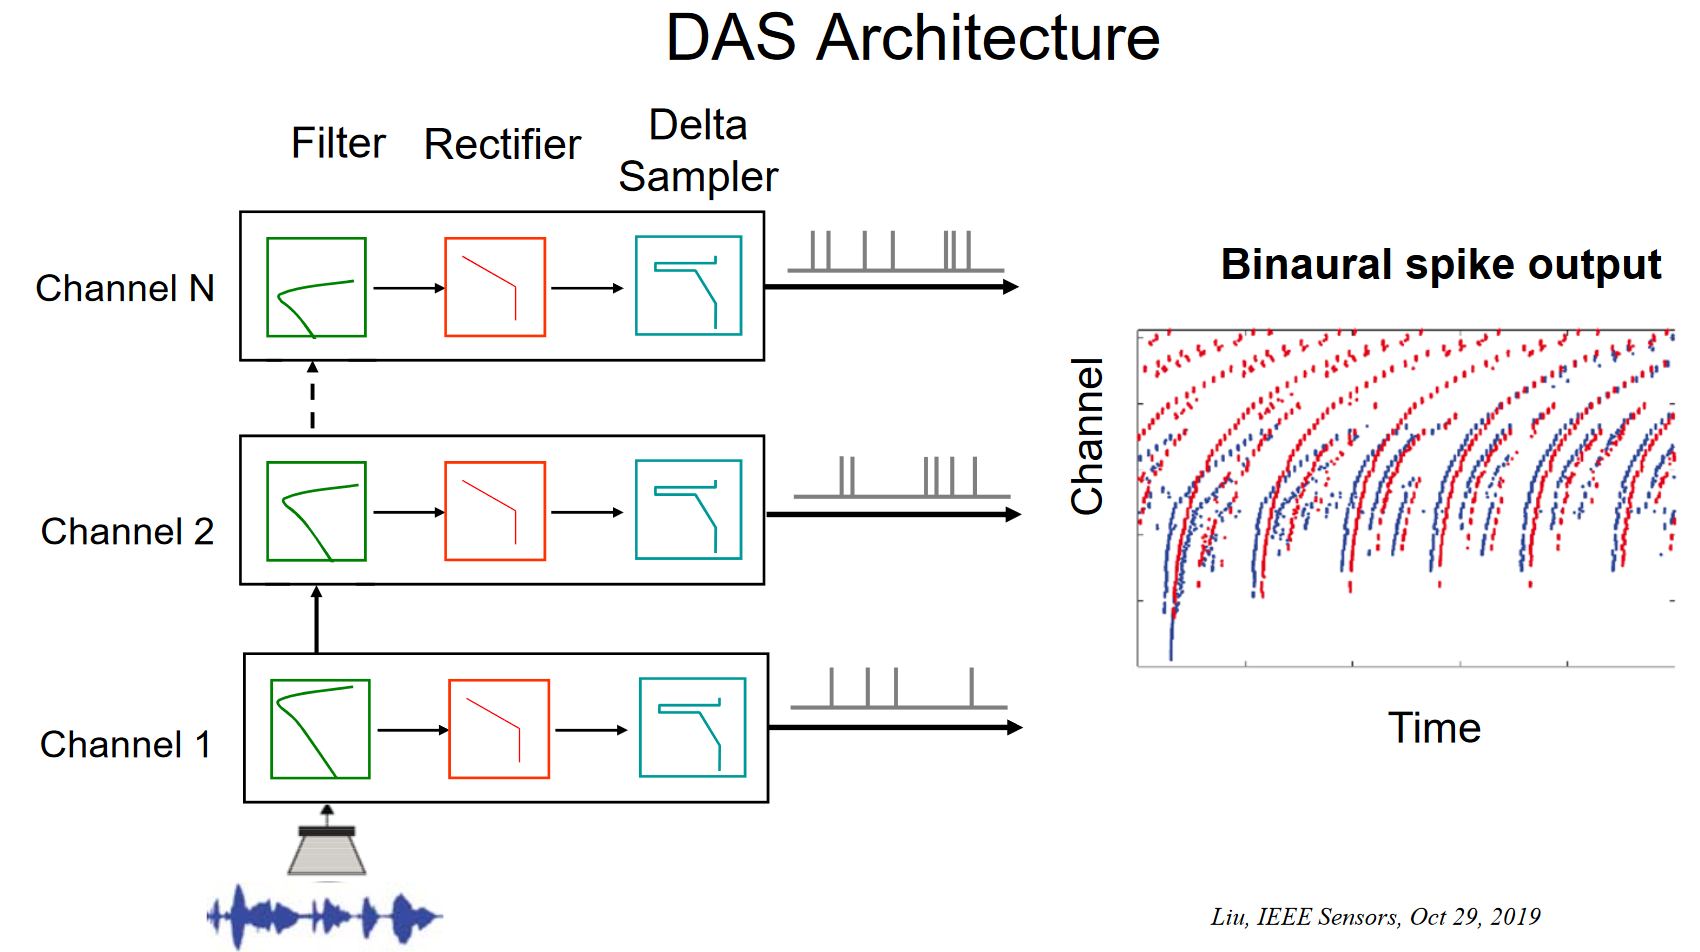
\includegraphics[width=0.8\linewidth]{11_NeuromorphicSystems1/figures/DAS.PNG}
    \caption{The DAS architecture.}
    \label{fig:dvs}
\end{figure}
%

\subsubsection{CAVIAR}
CAVIAR (Convolution AER VIsion Architecture for Real-time), was the largest multichip multilayer AER real-time, frame-free vision system (Figure 13.13) built at the time, with a combined total of 45K neurons and 5M synapses (Serrano-Gotarredonaet al. 2009). This system has four custom mixed-signal AER chips, five custom digital AER interface components and it performs up to 12G synaptic operations per second. It is capable of achieving millisecond object recognition and tracking latencies, illustrating the computational efficiency of AER systems. The CAVIAR vision system is composed of the following custom chips: the DVS temporal contrast retina chip, a set of programmable kernel convolution chips, a 2D winner-take-all (WTA) object chip, and a delay line chip and learning chip.

%
\begin{figure}[h]
    \centering
    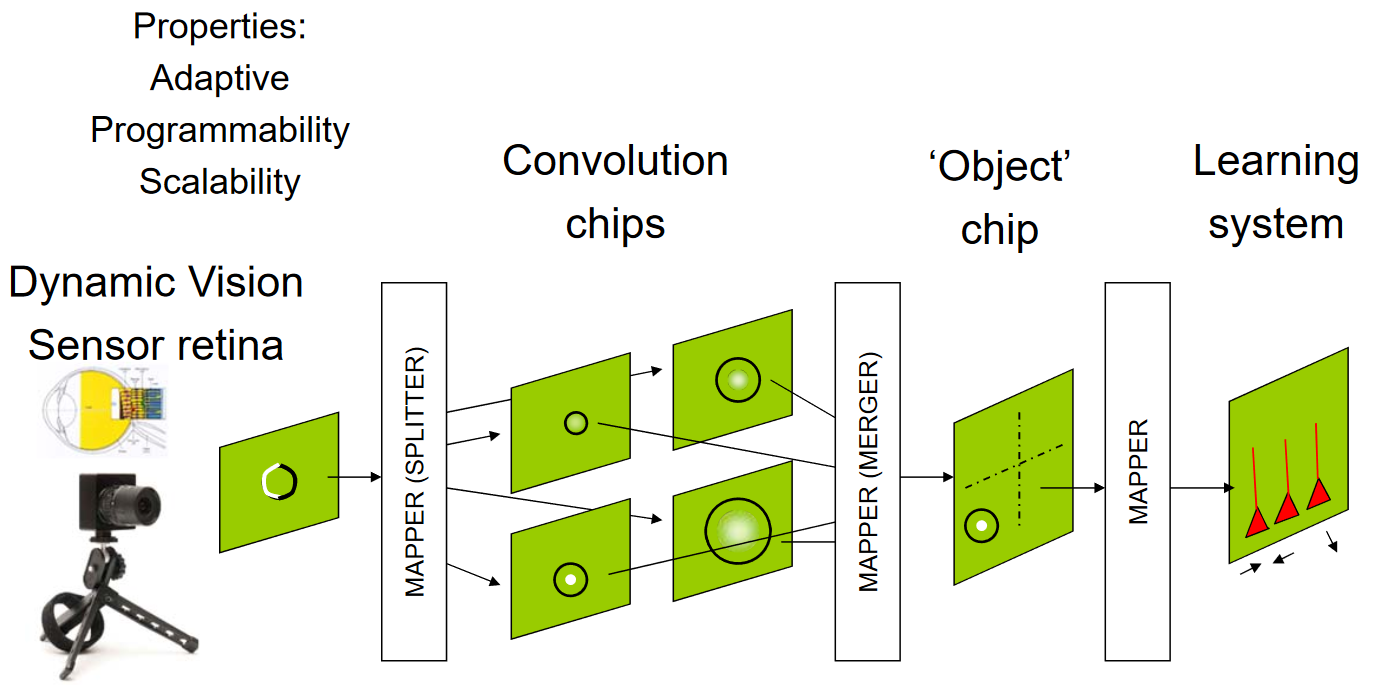
\includegraphics[width=0.8\linewidth]{11_NeuromorphicSystems1/figures/caviar.png}
    \caption{CAVIAR architecture.}
    \label{fig:dvs}
\end{figure}
%

\subsection{Sensors driving event-driven Deep Learning networks}
\subsubsection{Background of deep networks and biological aspirations}
Yann LeCun et al. (1989) used back-propagation to learn the convolution kernel coefficients directly from images of hand-written numbers. Learning was thus fully automatic, performed better than manual coefficient design, and was suited to a broader range of image recognition problems and image types. This was the origin of LeNet, a very well known 5-layer CNN model.

The DAVE project consists of a small off-road robot that uses an end-to-end learning system to avoid obstacles solely from visual input. The DAVE robot has two cameras with analog video transmitter. The video is transmitted to a remote computer that collects the data, runs the automatic driving system, and controls the robot through radio control. A convolutional network takes the left and right camera images (YUV components) and is trained to directly predict the steering angle of a human driver. The CNN ran at 10 FPS on 1.5GHz Celeron, was trained on about 90k frames. This led to DARPA LAGR program.

At the beginning of CNNs, everybody used threshold or sigmoid units, but cortical Firing frequency - Current (F-I) curves have a different look. To model this curve, biologists introduced Rectified Linear Units (ReLU) to ML, more than a decade before mainstream AI started using it. ReLU allows unbounded values to pass through while providing an essential non-linearity. It helps the back=propagation algorithm avoid the vanishing gradients problem and produces sparse feature maps.

The max-pooling operation is, in neuroscience terms, akin to a neuron’s firing rate being equal to the firing rate of its highest firing input, like in he well-known Winner-Takes-All networks. Because neurons pool from many neurons, it’s hard to devise a neuron that could straightforwardly do this. But the pooling operation was inspired by the discovery of complex cells and originally started as an averaging operation, something trivially achievable by neurons. Max-pooling, however, has been found to be more successful in terms of object recognition performance and fitting biological data and is now widely used. 

% [https://neurdiness.wordpress.com/2018/05/17/deep-convolutional-neural-networks-as-models-of-the-visual-system-qa/]

\subsubsection{Spiking sensors + deep network systems}

When interfacing neuromorphic sensors like the DAVIS or DAS with deep networks, a data-driven approach is used. In data-driven pipelines, processing is triggered only by input events so processing times, dissipation power and latencies can be reduced. Some examples of projects developed using this approach and neuromorphic sensors are the Predator and the RoShamBo.

The predator/prey robot consists of a CNN that is trained and run on data from a Dynamic and Active Pixel Sensor (DAVIS) mounted on a Summit XL robot (the predator), which follows another one (the prey). The CNN is driven by both conventional image frames and dynamic vision sensor "frames" that consist of a constant number of DAVIS ON and OFF events. The network is thus "data driven" at a sample rate proportional to the scene activity, so the effective sample rate varies from 15 Hz to 240 Hz depending on the robot speeds. 

RoShamBo is system which uses the DVS sensor to drive a 5-layer CNN into playing the game of rock-paper-scissors against a human. CNN input images are generated at a variable, data-driven rate between 1-200 Hz by accumulating asynchronous DVS address-events into 64x64 pixel 2D histograms of a constant total number of events. The DVS + NullHop is so fast that the symbol can be recognized as the person is opening it's hand. Thus the system shows the symbol to beat the human before they complete their throw.

\subsubsection{Data-driven deep networks: exploiting sparsity}


\textbf{NullHop} is a CNN accelerator that exploits the spatial sparsity of neuron activations to accelerate the computation and reduce memory requirements. The flexible architecture allows high utilization of available computing resources across kernel sizes ranging from 1x1 to 7x7. NullHop can process up to 128 input and 128 output feature maps per layer in a single pass. 

The accelerator implements one convolutional stage followed by a ReLU transformation and then a max-pooling stage. The ReLU and max-pooling stages can be disabled. To implement the full forward pass in a CNN, the accelerator evaluates convolutional stages one after another in a sequential manner. The input feature maps and the kernel values for the current convolutional layer are stored in two independent SRAM blocks. 

The input decoding block is able to directly skip over zero pixels in the compressed input feature maps without wasting any MAC operation. NullHop uses a novel sparse matrix compression algorithm allowing it to encode feature maps with 1.x bits/zero pixel, achieving superior memory usage.

\textbf{DeltaNet} is a Recurrent Neural Network (RNN) architecture in which each neuron transmits its value only when the change in its activation exceeds a threshold. RNNs require a large weight memory storage that is expensive to allocate to on-chip static random access memory (SRAM). The execution of RNNs as delta networks is attractive because their states must be stored and fetched at every time-step. By caching neuron activations, computations can be skipped where inputs change by a small amount from the previous update. The purpose of a delta network is to transform a dense matrix-vector multiplication (for example, a weight matrix and a state vector) into a sparse matrix-vector multiplication followed by a full addition. This transformation leads to savings on both operations (actual multiplications) and more importantly memory accesses (weight fetches).

A project which harnesses the power of DeltaNets is the hardware system for continuous speech recognition. It consists of a single-layer RNN with 256 gated recurrent unit (GRU) neurons and is driven by input features generated either from the output of a filter bank running on the ARM core of the FPGA in a PmodMic3 microphone setup or from the asynchronous outputs of a spiking silicon cochlea circuit. The microphone setup achieves 7.1 ms minimum latency and 177 frames-per-second (FPS) maximum throughput while the cochlea setup achieves 2.9 ms minimum latency and 345 FPS maximum throughput. The low latency and 70 mW power consumption of the DeltaRNN makes it suitable as an IoT computing platform.

\subsubsection{Conversion of deep ANN to deep SNN} [almost all from rueckauer et al.]
Inference in very large deep networks like GoogLeNet and VGG-16, requires substantial computational and energy costs, thus limiting their use in mobile and embedded applications. Recent work have shown that the event-based mode of operation in SNNs is particularly attractive for reducing the latency and computational load of deep neural networks. 

The most straight-forward way to combine the advantages of these models is to take the parameters of a pre-trained ANN and to map them to an equivalent-accuracy SNN. The basic principle of converting ANNs into SNNs is that firing rates $r_i^l$ of spiking neurons correlates with the its original graded activation $a_i^l$ of analog neurons. 

The spiking neuron integrates inputs $z^l_i(t)$ until the membrane potential $V^l_i(t)$ exceeds a threshold $V_{thr} \epsilon R^+$ and a spike is generated. Once the spike is generated, the membrane potential
is reset. Two types of reset are possible: reset the membrane potential back to a baseline, typically zero and reset by subtraction, or “linear reset
mode”, subtracts the threshold $V_{thr}$ from the membrane potential at the time when it exceeds the threshold:

\begin{equation}\label{eq}
    r^l_i(t) = \left\{
	\begin{array}{ll}
		\left(V_i^l(t-1)+z_i^ll(t)\right)(1-\Theta_{t,i}^l)  & \mbox{reset to zero} \\
		V_i^l(t-1)+z_i^ll(t)-V_{thr}\Theta_{t,i}^l) & \mbox{reset by subtraction}
	\end{array}
\right.
\end{equation}

The input to first-layer neurons is then related to the ANN activations via $z^l_i = V_{thr}\cdot a^l_i$. In order to relate these ANN activations to the SNN spike rates, an average is done on the membrane Equation \ref{eq} over the simulation time. The resulting rates are:
\begin{equation}
    r^l_i(t) = \left\{
	\begin{array}{ll}
		a^l_i r_{max}\cdot \frac{V_{thr}}{V_{thr}+\epsilon^l_i} - \frac{V^l_i(t)}{t\cdot (V_{thr}+\epsilon_i^l)} & \mbox{reset to zero} \\
		a^l_i r_{max} - \frac{V^l_i(t)}{t\cdot V_{thr}} & \mbox{reset by subtraction}
	\end{array}
\right.
\end{equation}

Some important operators of standard ANNs need a special treatment in the conversion process. 

In a spiking network, a \textbf{bias} can simply be implemented with a constant input current of equal sign as the bias. Alternatively, one could present the bias with an external spike input of constant rate proportional to the ANN bias.

The \textbf{data-based weight normalization} mechanism is based on the linearity of the ReLU unit used for ANNs. It can simply be extended to biases by linearly rescaling all weights and biases such that the ANN activation a is smaller than 1 for all training examples. Denoting the maximum ReLU activation in layer l as $\lambda^l = max[a^l]$, then weights $W^l$ and biases $b^l$ are normalized to $W^l \rightarrow W^l\frac{\lambda^{l-1}}{\lambda^l}$ and $b^l \rightarrow b^l/\lambda^l$.

The analog \textbf{input activations} are interpreted as constant currents. The input to the neurons in the first hidden layer is obtained by multiplying the corresponding kernels with the analog input image x:

\begin{equation}
    z_i^1 = V_{thr}\left(\sum_{j=1}^{M^0}W_{ij}^1 x_j+b_{i}^1\right)
\end{equation}

This results in one constant charge value $z_i^1$ per neuron i, which is added to the membrane potential at every time step. The spiking output then begins with the first hidden layer.

\textbf{Softmax} is commonly used on the outputs of a deep ANN, because it results in normalized and strictly positive class likelihoods. In this case output spikes are triggered by an external Poisson generator with fixed firing rate. To determine if a neuron should spike, we compute the softmax on the membrane potentials of all neurons, and use the resulting values in range of [0, 1] as rate parameters in a Poisson process for
each neuron.

The max-pooling operation mechanism is based on output units contain gating functions that only let spikes from the maximally firing neuron pass, while discarding spikes from other neurons. The gating function is controlled by computing estimates of the pre-synaptic firing rates, e.g., by computing an online or exponentially weighted average of these rates.

%
\begin{figure}[h]
    \centering
    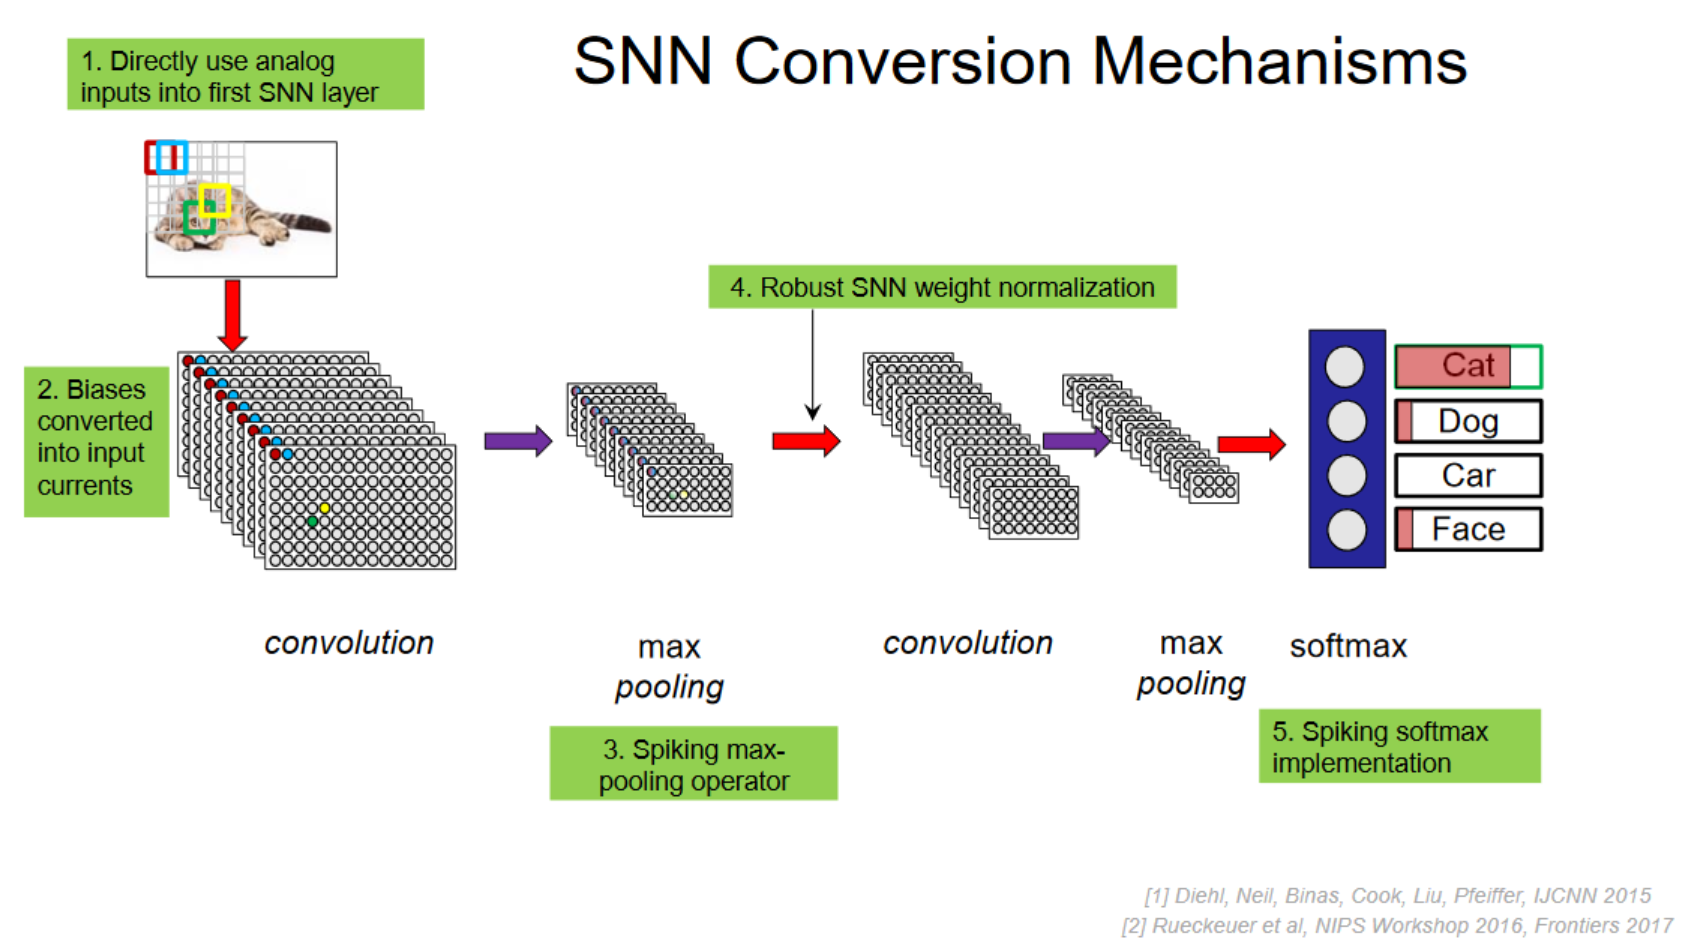
\includegraphics[width=0.8\linewidth]{11_NeuromorphicSystems1/figures/conversion.PNG}
    \caption{Converting different modules of ANNs into SNNs.}
    \label{fig:dvs}
\end{figure}
%

Alternatively, the converted SNN can be exported for use in spiking simulators like pyNN or
Brian2.
\end{document}